\documentclass[aspectratio=169]{beamer}

\usetheme{ucl}

\usepackage{amsmath,amsfonts,amsthm,bm}
\usepackage[detect-all]{siunitx}
\usepackage{hyperref}
\usepackage{subcaption}
\captionsetup[subfigure]{labelformat=empty}


\usepackage[T1]{fontenc}
% \usepackage{lmodern}
\renewcommand\sfdefault{uhv}
\usefonttheme[onlymath]{serif}


%%% Change the colour of the main banner
%%% The background should be one of the UCL colours (except pink or white):
%%%   black,darkpurple,darkred,darkblue,darkgreen,darkbrown,richred,midred,
%%%   navyblue,midgreen,darkgrey,orange,brightblue,brightgreen,lightgrey,
%%%   lightpurple,yellow,lightblue,lightgreen,stone
\setbeamercolor{banner}{bg=navyblue}
% \setbeamercolor{background canvas}{bg=lightgrey}
% \setbeamercolor{banner stripe}{bg=black}

\useoutertheme[small]{ucltitlebanner}
\setbeamersize{description width=2em}
\setbeamerfont{caption}{size=\tiny}

\beamertemplatenavigationsymbolsempty
% \setbeamerfont{page number in head/foot}{size=\large\bfseries}
\setbeamertemplate{footline}[frame number]

\title[Emittance measurement]{Simulating the Measurement of the \\ Electron Beam Emittance at AWAKE}
\author{Patrick Chin}
\institute[UCL]{%
	Supervisor: Prof Matthew Wing \\[1em]
	Department of Physics and Astronomy \\
	University College London
}

\begin{document}

\begin{frame}
  \titlepage
\end{frame}

\begin{frame}{The AWAKE project}
	\begin{columns}
		\begin{column}{.5\linewidth}
			\begin{itemize}
				% \item Goal to accelerate an electron beam to the TeV regime
				\item Scaling RF accelerators is impractical: %
					\begin{itemize}
						\item synchrotron radiation
						\item cost
						% \item Energy loss due to synchrotron radiation
						% \item Cost of building a linear accelerator tens of km long
					\end{itemize}
				\item Plasma wakefield acceleration is an alternative
					\begin{itemize}
						\item Larger EM
							gradients (up to the GV/m scale)
						\item Electrons will be accelerated in the wakefield
							of a proton beam
						% \item Plasmas are able to sustain much larger EM
						% 	gradients (up to the GV/m scale)
						% \item Electrons will be accelerated in the wakefield
						% 	of a proton beam
					\end{itemize}
				\item AWAKE is a proof-of-concept
			\end{itemize}
		\end{column}
		\begin{column}{.5\linewidth}
			\begin{figure}[h]
				\centering
				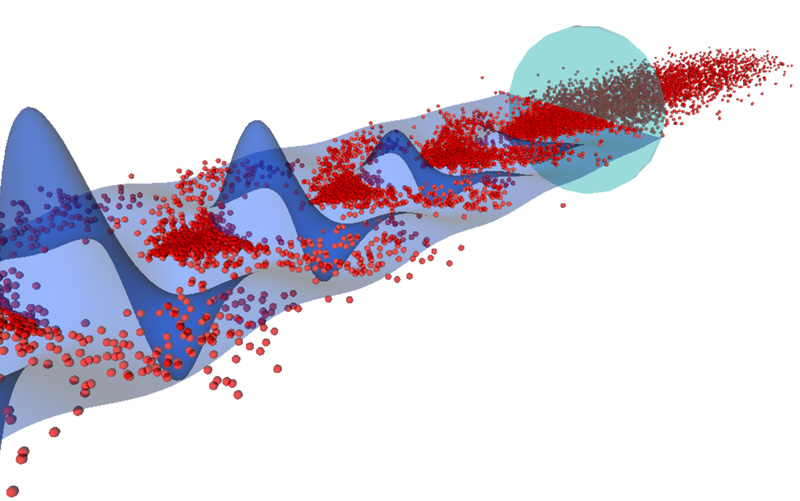
\includegraphics[width=\linewidth]{./wakefield_artist.jpg}
				\caption{Artists impression of the AWAKE witness beam electrons
				(red) captured and accelerated by the plasma wakefield (blue).
				Credit: Alexey Petrenko / CERN. \url{https://www.hep.ucl.ac.uk/awake/}}
			\end{figure}
		\end{column}
	\end{columns}

\end{frame}

\begin{frame}{The Spectrometer}
	\begin{columns}
		\begin{column}{0.6\linewidth}
			Goals:
			\begin{enumerate}
				% there are two main goals for the spectrometer
				\item Measure the energy distribution of the beam
					% as the energy of the beam defines the success of the
					% experiment
				\item Determine the quality of the beam
					% which can be quantified by the emittance
			\end{enumerate}
			\vspace{1em}
			Objective:\\
			\hspace*{18pt} Investigate the effect on the emittance measurement of
			experimental parameters:
			\begin{itemize}
				\item mean energy and energy spread
				\item background photons
				\item emittance
			\end{itemize}
		\end{column}
		\begin{column}{0.4\linewidth}
			\begin{figure}[h]
				\centering
				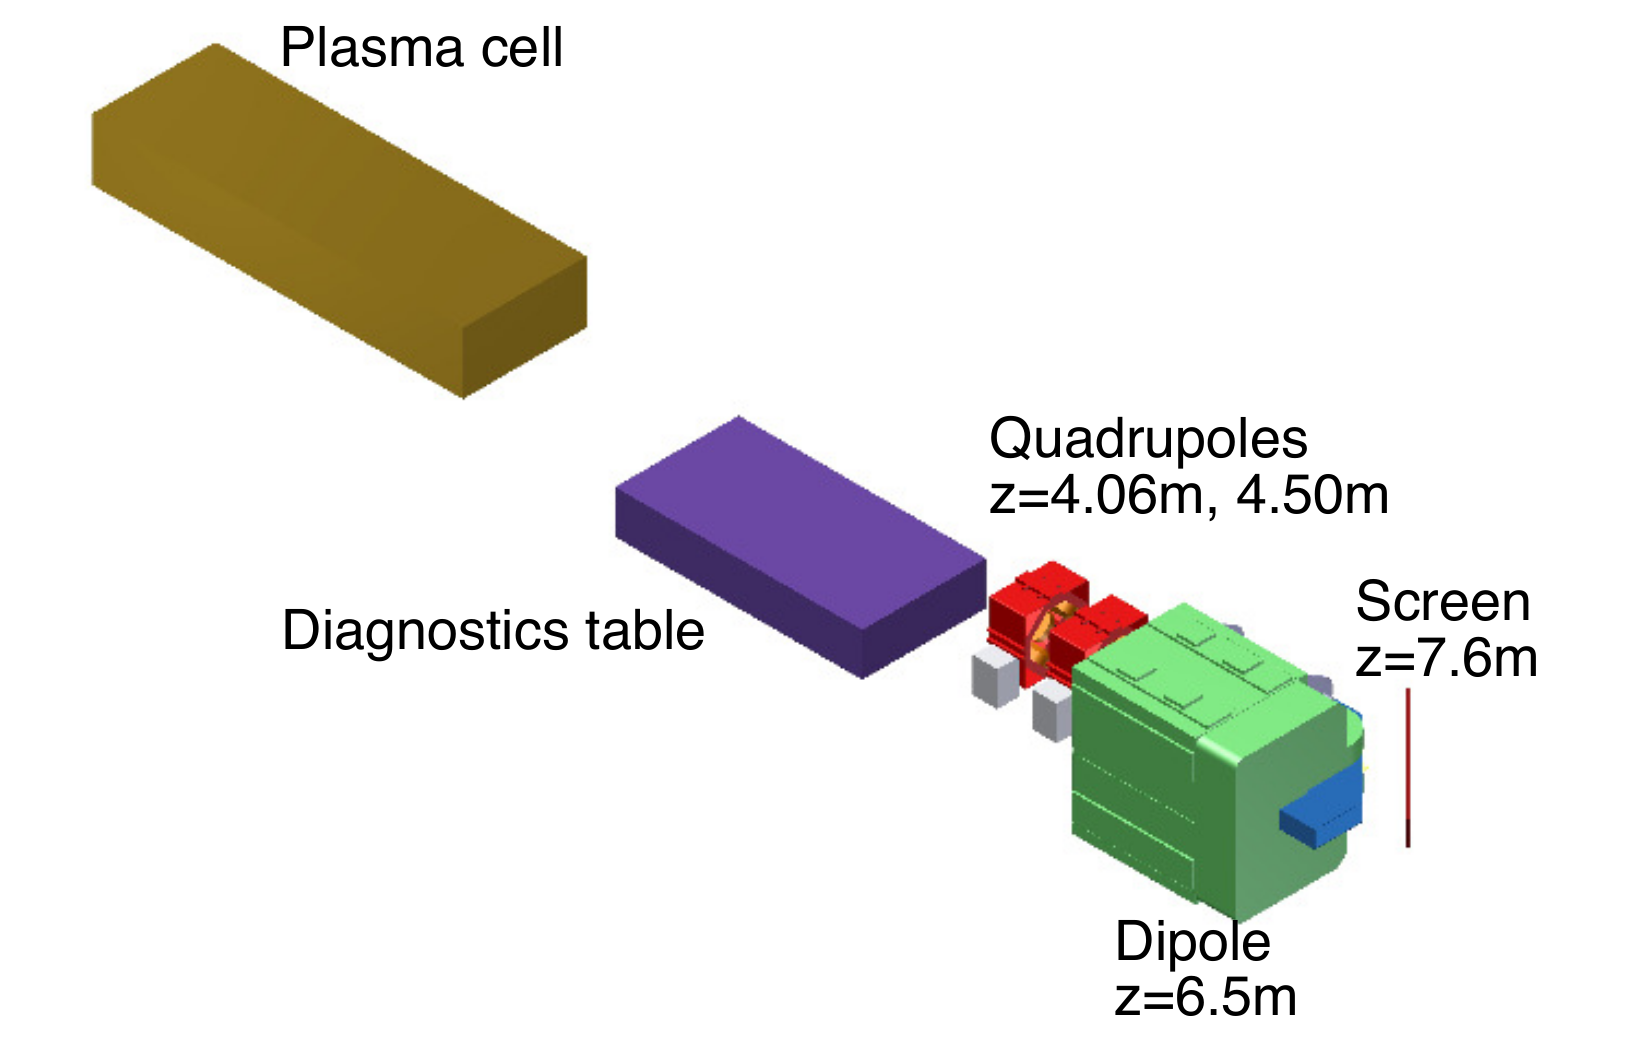
\includegraphics[width=\linewidth]{spectrometer}
				\caption{
					3D schematic of the spectrometer downstream of the
					plasma cell. Source: Deacon, Lawrence, et al. "Development of a
					spectrometer for proton driven plasma wakefield accelerated
					electrons at AWAKE." (2015): WEPWA045.
				}
			\end{figure}
		\end{column}
	\end{columns}
\end{frame}

\small
\begin{frame}{The Simulation}

	To simulate the shape of the beam on the screen the following transport
	matrix $\mathcal{M}$ is applied to the input beam matrix $\bm{\sigma_0}$

	\begin{align*}
		\bm{\sigma}_1 &=
		\epsilon
		\begin{pmatrix}
			\beta & -\alpha \\
			-\alpha & \gamma
		\end{pmatrix} =
		\mathcal{M}\;\bm{\sigma}_0\;\mathcal{M}^T, \quad
		% \text{where}\quad
		\epsilon = \sqrt{\det{\bm{\sigma}}}, \quad
		\beta\gamma-\alpha^2=1, \quad
		\tan2\varphi = \tfrac{2\alpha}{\gamma-\beta}
		\\[1em] %
		\mathcal{M} &= \underbrace{
		\begin{pmatrix}
			1 & d \\
			0 & 1
		\end{pmatrix}}_\text{drift}
		\cdot
		\underbrace{
		\begin{pmatrix}
			\cos\varphi_1 & \tfrac{\sin\varphi_1}{\sqrt{k_1}} \\
			-\sqrt{k_1}\sin\varphi_1 & \cos\varphi_1
		\end{pmatrix}}_\text{vertically focusing quadrupole}
		\cdot
		\underbrace{
		\begin{pmatrix}
			1 & g_1 \\
			0 & 1
		\end{pmatrix}}_\text{gap}
		\cdot
		\underbrace{
		\begin{pmatrix}
			\cosh\varphi_2 & \tfrac{\sinh\varphi_2}{\sqrt{|k_2|}} \\
			-\sqrt{k_2}\sinh\varphi_2 & \cosh\varphi_2
		\end{pmatrix}}_\text{horizontally focusing quadrupole}
		\cdot
		\underbrace{
		\begin{pmatrix}
			1 & g_2 \\
			0 & 1
		\end{pmatrix}}_\text{gap}
	\end{align*}
	\\[1em]

	where quadrupole strength $k_1$ and $k_2$ and drift distance to screen $d$
	are functions of energy.\\
	From this we are able to derive a function \(\sigma_y \left(x;
	\beta,\gamma,\epsilon \right)\) where\\

	% \vspace*{-1.0em}
	\begin{align*}
		\sigma_y = \sqrt{\bm{\sigma}_{1,11}} = \sqrt{\epsilon\beta}
		&\qquad\text{rms beam envelope} \\
		% \sigma_{y'} = \sqrt{\bm{\sigma}_{1,22}} = \sqrt{\epsilon\gamma}
		% &\qquad\text{rms beam divergence}
	\end{align*}
\end{frame}

\begin{frame}{Beam Reconstruction Examples}
	% here are two examples
	\begin{figure}
		\centering
		\vspace*{-2.5em}
		\begin{subfigure}{0.3333\textwidth}
			\centering
			\includegraphics[width=\linewidth]{./output/run-pespread-old/pespread_0.3/n1/graph.pdf}
			\caption{\tiny
				\begin{tabular}{r|l}
					$\bar{E}  $  & \SI{1.3}{\giga\electronvolt} \\
					$\sigma_E $  & \SI{0.4}{\giga\electronvolt} \\
					$\epsilon $  & \SI{1e-6}{\meter\radian} \\
					bg factor    & 1
				\end{tabular}
			}
		\end{subfigure}%
		~
		\begin{subfigure}{0.3333\textwidth}
			\centering
			\includegraphics[width=\linewidth]{./output/run-pespread-old/pespread_0.01/n1/graph.pdf}
			\caption{\tiny
				\begin{tabular}{r|l}
					$\bar{E}  $  & \SI{1.3}{\giga\electronvolt} \\
					$\sigma_E $  & \SI{0.013}{\giga\electronvolt} \\
					$\epsilon $  & \SI{1e-6}{\meter\radian} \\
					bg factor    & 1
				\end{tabular}
			}
		\end{subfigure}%
		~
		\begin{subfigure}{0.3333\textwidth}
			\centering
			\includegraphics[width=\linewidth]{./output/run-bgdens/bgphotons_7000/n1/graph.pdf}
			\caption{\tiny
				\begin{tabular}{r|l}
					$\bar{E}  $  & \SI{1.3}{\giga\electronvolt} \\
					$\sigma_E $  & \SI{0.4}{\giga\electronvolt} \\
					$\epsilon $  & \SI{1e-6}{\meter\radian} \\
					bg factor  & 7000
				\end{tabular}
			}
		\end{subfigure}%
	\end{figure}

	\begin{itemize}
		% \scriptsize
		\item Black line: the function \(\sigma_y \left(x; \beta,\gamma,\epsilon \right)\)
		\item Black points: measured rms of the vertical beam spread for each
			column of pixels
		\item Blue line: the function \(\sigma_y \left(x; \beta,\gamma,\epsilon \right)\)
			fitted to the points
	\end{itemize}

	% To fit the
\end{frame}

\begin{frame}[t]{Results}
	\framesubtitle{Energy Spread}
	The effect of the energy spread of the electron beam on the simulated
	emittance measurement.

	\begin{figure}
		\vspace*{-1em}
		\begin{subfigure}[t]{0.45\textwidth}
			\centering
			% \includegraphics[width=0.83\linewidth]{./output/run-pespread/emit_vs_pespread.pdf}
			\includegraphics[scale=0.7]{./output/run-pespread/emit_vs_pespread.pdf}
		\end{subfigure}%
		~
		\begin{subfigure}[t]{0.55\textwidth}
			\centering
			\includegraphics[scale=0.7]{./output/run-pespread2/emit_vs_pespread.pdf}
		\end{subfigure}
	\end{figure}

	For lower energy spreads, the electron beam is spread much smaller
	accross the screen.
\end{frame}

\begin{frame}[t]{Results}
	\framesubtitle{Background Photons}
	The effect of background photons on the simulated emittance measurement.\\

	\begin{figure}[!t]
		\centering
		\vspace*{-1em}
		\begin{subfigure}[t]{0.45\textwidth}
			\centering
			\includegraphics[scale=0.7]{./output/run-bgdens/emit_vs_bgdens.pdf}
		\end{subfigure}%
		~
		\begin{subfigure}[t]{0.55\textwidth}
			\centering
			\includegraphics[scale=0.7]{./output/run-bgdens2/emit_vs_bgdens.pdf}
		\end{subfigure}%
		% \begin{subfigure}[t]{0.5\textwidth}
		% 	\centering
		% 	% \includegraphics[width=0.8\linewidth]{emitperr_vs_bgdens.pdf}
		% 	\includegraphics[scale=0.7]{./output/run-bgdens/emitperr_vs_bgdens.pdf}
		% \end{subfigure}
	\end{figure}

	The number of photons per bin is expected to be in the order of magnitude of \num{1e-2}.
	% As the photon density increases 
\end{frame}

\begin{frame}{Results}
	\framesubtitle{Input Emittance}
	The effect of the emittance on the simulated emittance measurement.\\
	\begin{figure}
		\centering
		% \vspace*{-0.9em}
		\begin{subfigure}[b]{0.45\textwidth}
			\centering
			% \includegraphics[width=0.8\linewidth]{emitr_vs_inemit.pdf}
			% \includegraphics[width=0.8\linewidth]{./output/run-inemit/emitr_vs_inemit.pdf}
			\includegraphics[scale=0.7]{./output/run-inemit/emitr_vs_inemit.pdf}
		\end{subfigure}%
		% ~
		% \begin{subfigure}[b]{0.5\textwidth}
		% 	\centering
		% 	\includegraphics[width=\linewidth]{./output/run-inemit/emit_7e-5/n1/graph.pdf}
		% \end{subfigure}
		~
		\begin{subfigure}[b]{0.55\textwidth}
			\centering
			\includegraphics[scale=0.7]{./output/run-inemit2/emitr_vs_inemit.pdf}
		\end{subfigure}
	\end{figure}

	For large emittances, many of the electrons completely miss the screen so
	we arrive at a lower value for the transverse momenta of the beam.
\end{frame}

\begin{frame}{Conclusion}
	\begin{itemize}
		\item Shown how the energy spread, background and emittance, affect the
			emittance measurement.
		\item Graphs are quite specific and are only accurate when
			keeping certain parameters constant.
		\item Give a general idea as to how the emittance measurement should
			behave with respect to each parameter.
		\item This should help 
	\end{itemize}
	\vfill
	\centering
	Thanks for listening!
\end{frame}

\end{document}

